\subsection{Decorator}
\begin{flushleft}
    \textbf{Decorator} là một mẫu thiết kế cấu trúc cho phép mở rộng hoặc thêm chức năng mới cho một đối tượng động mà không làm thay đổi trực tiếp lớp của nó. `Decorator' hoạt động bằng cách bọc (wrap) đối tượng gốc, sau đó tùy chỉnh hoặc mở rộng hành vi của nó.
\end{flushleft}

\subsubsection{Vấn đề}
\begin{itemize}
    \item Hãy tưởng tượng bạn đang làm việc với một hệ thống xử lý đơn hàng thương mại điện tử. Ban đầu, hệ thống này rất đơn giản: mỗi đơn hàng chỉ chứa danh sách các sản phẩm và thông tin thanh toán cơ bản. Mọi thứ đều theo một quy trình mặc định, từ thanh toán đến vận chuyển tiêu chuẩn, không có tùy chọn bổ sung nào khác.
    \item Mọi thứ vẫn vận hành suôn sẻ cho tới khi khách hàng đưa ra các yêu cầu mới:
          \begin{itemize}
              \item \textit{`Tôi muốn đơn hàng được giao hỏa tốc vì tôi cần nó ngay bây giờ'}
              \item \textit{`Sản phẩm này là một món quà, hãy đóng gói thật đẹp giúp tôi'}
              \item \textit{`Hàng của tôi dễ vỡ, tôi muốn thêm bảo hiểm để đảm bảo an toàn'}
              \item \ldots
          \end{itemize}
    \item Bạn cố gắng cập nhật hệ thống để đáp ứng các yêu cầu này bằng cách thêm các thuộc tính mới vào lớp đơn hàng (như \textit{isGiftWrap, isExpressDelivery, hasInsurance\ldots}).\newline~Tuy nhiên điều này nhanh chóng trở nên phức tạp bởi vì:
          \begin{itemize}
              \item Mỗi yêu cầu bổ sung dẫn đến thêm nhiều điều kiện \textit{if-else} vào mã nguồn.
              \item Các phương thức xử lý đơn hàng trở nên cồng kềnh và khó bảo trì.
              \item Khi số lượng dịch vụ bổ sung tăng lên, việc tổ hợp các tùy chọn trở thành một cơn ác mộng.
          \end{itemize}
    \item Lúc này, bạn nhận ra cần một cách tiếp cận tốt hơn để mở rộng chức năng của đơn hàng mà không làm phức tạp thêm cấu trúc lớp gốc.
\end{itemize}

\subsubsection{Mục đích}
\begin{itemize}
    \item Để giải quyết vấn đề được đặt ra, bạn bắt đầu nghĩ đến kế thừa (Inheritance) để thay đổi lớp ban đầu. Tuy nhiên kế thừa lại có một số hạn chế như sau:
          \begin{itemize}
              \item \textbf{Tính chất tĩnh:} Hành vi được xác định tại thời điểm biên dịch, khó thay đổi khi chạy.
              \item \textbf{Không hỗ trợ đa kế thừa:} Nhiều ngôn ngữ lập trình không cho phép đa kế thừa, hạn chế khả năng mở rộng.
          \end{itemize}

    \item Bạn tiếp tục tìm đến những giải pháp khác là tập hợp (Aggregation) hoặc thành phần (Composition) để khắc phục nhược điểm của kế thừa:
          \begin{itemize}
              \item Cho phép đối tượng tham chiếu và ủy quyền nhiệm vụ cho các đối tượng khác.
              \item Thay đổi hành vi linh hoạt tại thời điểm chạy.
          \end{itemize}
    \item Hai nguyên tắc này nền tảng cho nhiều mẫu thiết kế, đặc biệt là \verb|Decorator Pattern|.
\end{itemize}

\subsubsection{Giải pháp}
\begin{enumerate}
    \item \textbf{Cơ chế của Decorator}\newline
          \textit{Decorator Pattern} mở rộng hành vi bằng cách `bọc' đối tượng trong các lớp mở rộng, mỗi lớp thêm hoặc thay đổi chức năng mà không ảnh hưởng đến đối tượng gốc.
          \begin{itemize}
              \item \textbf{Tham chiếu đối tượng gốc:} Các lớp Decorator chứa tham chiếu đến đối tượng cần bọc (có thể là đối tượng cơ bản hoặc một Decorator khác).
              \item \textbf{Giao diện thống nhất:} Decorator và đối tượng gốc tuân theo cùng một giao diện hoặc lớp trừu tượng. Điều này giúp Decorator có thể thay thế đối tượng gốc mà không làm thay đổi logic tổng thể.
              \item \textbf{Thêm hành vi từng bước:} Decorator thực hiện logic riêng trước hoặc sau khi gọi phương thức của đối tượng bọc.
              \item \textbf{Kết hợp các tính năng:}
                    \begin{itemize}
                        \item Đơn hàng cơ bản: sử dụng \textit{BasicOrder}.
                        \item Đơn hàng cần gói quà và vận chuyển nhanh: sử dụng \textit{GiftWrapDecorator} và \textit{ExpressDeliveryDecorator} bọc quanh \textit{BasicOrder}.
                    \end{itemize}
          \end{itemize}

    \item \textbf{Ứng dụng vào hệ thống xử lý đơn hàng}
          \begin{itemize}
              \item \textbf{Đối tượng cơ bản:} \textit{BasicOrder} là đơn hàng tiêu chuẩn, chỉ chứa thông tin sản phẩm, chi phí cơ bản và mã giảm giá.
              \item \textbf{Thêm Decorator theo yêu cầu:}
                    \begin{itemize}
                        \item \textit{GiftWrapDecorator}: Thêm phí và mô tả gói quà.
                        \item \textit{ExpressDeliveryDecorator}: Thêm phí và đơn vị giao hàng nhanh.
                    \end{itemize}
              \item \textbf{Xử lý tuần tự:} Khi gọi phương thức như \verb|calculateTotal()|, mỗi lớp Decorator sẽ thêm logic riêng, sau đó chuyển lời gọi tới lớp tiếp theo, tạo nên một luồng xử lý linh hoạt và có tổ chức.
          \end{itemize}
\end{enumerate}

\subsubsection{Cấu trúc}
\begin{flushleft}
    \begin{enumerate}
        \item \textbf{Order:} Đây là một giao diện (interface) xác định các hành vi cơ bản của một đơn hàng, bao gồm tính toán tổng tiền và đặt hàng.
        \item \textbf{BasicOrder:} Lớp cụ thể thực hiện giao diện \verb|Order|, đại diện cho một đơn hàng cơ bản. Lớp này có các thuộc tính như tổng giá trị giỏ hàng, mã giảm giá và các phương thức để tính toán tổng tiền và đặt hàng.
        \item \textbf{OrderDecorator:} Đây là một lớp trừu tượng (abstract class) đóng vai trò là lớp cơ sở cho các lớp `decorator'. Lớp này có một thuộc tính tham chiếu đến một đối tượng \verb|Order| khác (\verb|wrappedOrder|) và các phương thức để tính toán tổng tiền và đặt hàng. Các phương thức này thường sẽ gọi đến các phương thức tương ứng của \verb|wrappedOrder| và thực hiện thêm các logic của các `decorator' khác.
        \item \textbf{ExpressDeliveryDecorator:} Lớp cụ thể kế thừa từ \verb|OrderDecorator|, đại diện cho một lớp `decorator' thêm chức năng giao hàng nhanh cho đơn hàng. Lớp này có các thuộc tính như nhà cung cấp giao hàng, phí giao hàng và các phương thức để tính toán tổng tiền bao gồm cả phí giao hàng và cập nhật nhà cung cấp giao hàng.
    \end{enumerate}

    \begin{figure}[H]
        \centering
        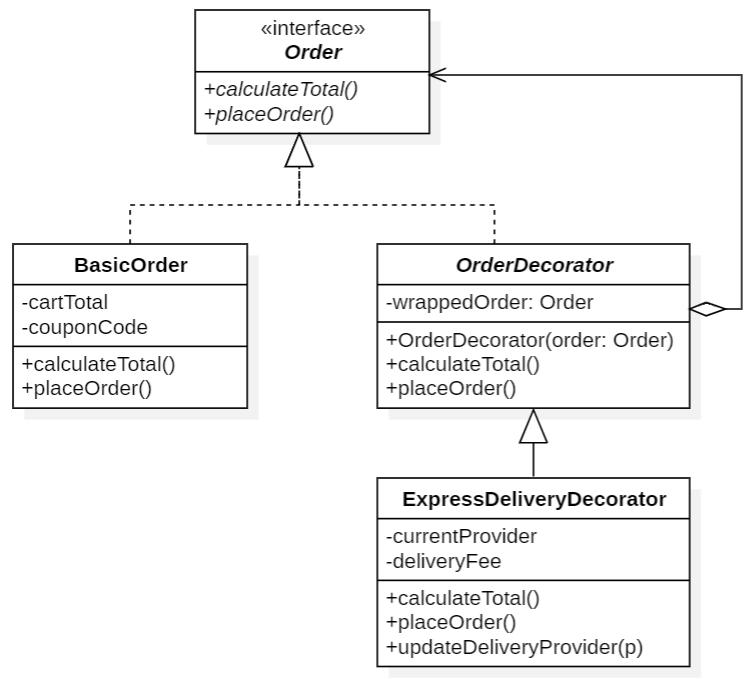
\includegraphics[width=0.9\textwidth]{../assets/screenshots/uml/decorator.png}
        \caption{Decorator Pattern UML Class Diagram}
    \end{figure}
\end{flushleft}

\subsubsection{Hoạt động}
\begin{flushleft}
    \begin{itemize}
        \item \textbf{Tạo đối tượng BasicOrder:} Đầu tiên, chúng ta tạo một đối tượng \verb|BasicOrder| để đại diện cho một đơn hàng cơ bản.
        \item \textbf{Decorator:} Sau đó, chúng ta có thể tạo các đối tượng \verb|OrderDecorator| để `trang trí' cho đối tượng \verb|BasicOrder|. Ví dụ, chúng ta tạo một đối tượng \verb|ExpressDeliveryDecorator| và truyền đối tượng \verb|BasicOrder| vào trong constructor của nó.
        \item \textbf{Gọi phương thức:} Khi gọi các phương thức của đối tượng được trang trí (ví dụ: \verb|calculateTotal()|), các phương thức này sẽ gọi đến các phương thức tương ứng của đối tượng được gói bên trong (BasicOrder) và thực hiện thêm các logic trang trí. Trong trường hợp của \verb|ExpressDeliveryDecorator|, phương thức \verb|calculateTotal()| sẽ tính toán tổng tiền của đơn hàng cơ bản và cộng thêm phí giao hàng.
    \end{itemize}
\end{flushleft}

\subsubsection{Khả năng ứng dụng}
\begin{flushleft}
    \begin{itemize}
        \item \textbf{Tạo ra các loại đơn hàng đa dạng:}
              \begin{itemize}
                  \item \textbf{BasicOrder:} Đơn hàng tiêu chuẩn, chỉ chứa thông tin sản phẩm, chi phí cơ bản và mã giảm giá.
                  \item \textbf{ExpressDeliveryDecorator(BasicOrder):} Đơn hàng với giao hàng nhanh, có thêm phí và đơn vị giao hàng.
              \end{itemize}
        \item \textbf{Linh hoạt và mở rộng:} Để thêm một tính năng mới (ví dụ: gói quà), chỉ cần tạo một lớp decorator mới kế thừa từ OrderDecorator và triển khai logic thêm tính năng đó.
        \item \textbf{Tách biệt mối quan tâm:} Mỗi lớp decorator chỉ tập trung vào một tính năng cụ thể, giúp code dễ đọc, dễ bảo trì và dễ kiểm thử hơn.
    \end{itemize}
\end{flushleft}

\subsubsection{Ưu nhược điểm}
\begin{enumerate}
    \item \textbf{Ưu điểm}
          \begin{itemize}
              \item \textbf{Linh hoạt:} Dễ dàng thêm các tính năng mới cho một đối tượng mà không cần thay đổi lớp gốc.
              \item \textbf{Mở rộng:} Có thể kết hợp nhiều lớp trang trí để tạo ra các hành vi phức tạp.
              \item \textbf{Tái sử dụng:} Các lớp trang trí có thể được tái sử dụng cho nhiều loại đối tượng khác nhau.
          \end{itemize}
    \item \textbf{Nhược điểm}
          \begin{itemize}
              \item Việc loại bỏ một lớp Decorator cụ thể trong ngăn xếp không đơn giản.
              \item Hành vi của Decorator phụ thuộc vào thứ tự áp dụng.
              \item Việc có cấu trúc lớp phức tạp và khó khăn trong việc xác định hành vi của đối tượng khiến việc đọc hiểu mã nguồn trở nên khó khăn.
          \end{itemize}
\end{enumerate}

\subsubsection{Mã nguồn}
\codeimport{cpp}{../src/ecommerce-demo/Order.hpp}
